\documentclass[letter,12pt]{article}
\usepackage{newtxtext,newtxmath, amsmath, amsfonts, bm,mathtools}
\usepackage{paralist, url, natbib, parskip}
\usepackage{adjustbox, todonotes} % , 
\usepackage{graphicx, subfig, rotating, booktabs, multirow}
\usepackage[makeroom]{cancel}
\usepackage[section]{placeins}
\usepackage[linesnumbered,lined,boxed,commentsnumbered]{algorithm2e}
\usepackage{xcolor, tikz}
\usetikzlibrary{decorations.markings}
\usetikzlibrary{patterns}
%\usepackage[margin=1.5cm, bottom=2cm]{geometry}
\usepackage[margin=3cm]{geometry}
\usepackage[margin=2cm]{caption}
\usepackage{titling}
\usepackage{setspace}
\DeclareCaptionStyle{italic}[justification=centering]{labelfont={bf},textfont={it},labelsep=colon}
\captionsetup[figure]{style=italic,format=hang,singlelinecheck=true}
\providecommand{\keywords}[1]{\textbf{\textit{Key words---}} #1}

\SetKwInOut{Parameter}{parameter}
\setlength{\algomargin}{2em}
\renewcommand{\familydefault}{ptm}
\newcommand{\dist}{\text{dist}}
\newcommand{\Null}{\text{Null}}
\newcommand{\diag}{\text{diag}}
\DeclareMathOperator{\sign}{sign}
\mathtoolsset{showonlyrefs}

\graphicspath{{./Graphics/}}

\allowdisplaybreaks
\onehalfspacing

% =======================================================================
\begin{document}
% =======================================================================
\tikzset{->-/.style={decoration={
  markings,
  mark=at position #1 with {\arrow{>}}},postaction={decorate}}}


\title{Leave-one-out kernel density estimates for outlier detection}
\author{Sevvandi Kandanaarachchi$^1$, Rob J. Hyndman$^2$}
\date{%
   \scriptsize{ $^1$ School of Science,  Mathematical Sciences, RMIT University, Melbourne VIC 3000, Australia.\\ 
   $^2$Department of Econometrics and Business Statistics, Monash University, Clayton VIC 3800, Australia.\\ [2ex]}%
    }
\begin{titlingpage}
\maketitle

\begin{abstract}
For later. 
\end{abstract}

\begin{keywords}outlier detection, leave-one-out kernel density estimate, topological data analysis
\end{keywords}

\end{titlingpage}

\newgeometry{top=1.5cm,bottom=2cm,right=1.5cm,left=1.5cm}
% =======================================================================
\section{Introduction}\label{sec:introduction}
% =======================================================================
% =======================================================================
\section{Methodology}\label{sec:methodology}
% =======================================================================
% =======================================================================
\subsection{Topological data analysis and persistent homology}\label{subsec:tda}
%This section gives an introduction to topological data analysis. 
Topological data analysis is the study of data using topological constructs. It is about inferring high dimensional structure from low dimensional representations such as points, and assembling discrete points to global structure \citep{ghrist2008barcodes}. Persistent homology is a method in algebraic topology that computes topological features of a space that persist across multiple scales or spatial resolutions. These features include connected components, topological circles and trapped volumes.  Features that persist for a wider range of spatial resolutions represent robust, intrinsic features of the data while features that sporadically change are perturbations resulting from noise. Persistent homology has been used in a wide variety of applications including biology  \citep{topaz2015topological}, computer graphics \citep{carlsson2008local} and engineering \citep{perea2015sliding}.

\subsubsection{Simplicial Complex}\label{subsubsec:simplicialcomplex}
A data cloud, represented as a collection of points, is used to construct a graph where the points are considered vertices and the edges are determined by the distance between the points. Given a proximity parameter $\epsilon$ two vertices are connected by an edge if the distance between these two points are less than or equal to $\epsilon$. Starting from this graph a simplicial complex -- a space built from simple pieces -- is constructed. A simplicial complex is a finite set of $k$-simplices, where $k$ denotes the dimension. To give some examples, a point is a $0$-simplex, an edge a $1$-simplex, a triangle a $2$-simplex and a tetrahedron a $3$-simplex. Suppose $S$ denotes a simplicial complex, which includes a $k$-simplex $\gamma$. Then all non-empty subsets of $\beta \subset \gamma$ are also included in $S$. For example if $S$ contains a triangle $pqr$, then the edges $pq$, $qr$ and $rs$, and the vertices $p$, $q$ and $r$ are also in $S$. 

Two types of $k$-simplices are the \textit{Vietoris-Rips} complex and the \textit{Cech} complex. We will construct a Vietoris-Rips complex from the data cloud. Given a set of points and a proximity parameter $\epsilon > 0$, $k+1$ points within a distance of $\epsilon$ to each other forms a $k$-simplex.  For example consider 5 points $p$, $q$, $r$, $s$ and $t$ and suppose the distance between any two points except $t$ is less than $\epsilon$. Then we can construct the edges $pq$, $pr$, $ps$, $qr$, $qs$ and $rs$. From the edges $pq$, $qr$ and $rp$ we can construct the triangle $pqr$, from $pq$, $qs$ and $sp$ the triangle $pqs$ and so on. By constructing the $4$ triangles $pqr$, $qrs$, $rsp$ and $spq$ we can construct the tetrahedron $pqrs$. The vertex $t$ is not connected to this $3$-simplex because the distance between $t$ and the other vertices is greater than $\epsilon$. As such, the simplicial complex resulting from these 5 points consist of the tetrahedron $pqrs$ and all the subset $k$-simplices and the vertex $t$. Figure~\ref{fig:tetrahedron} shows this simplicial complex. 

\begin{figure}
    \centering
    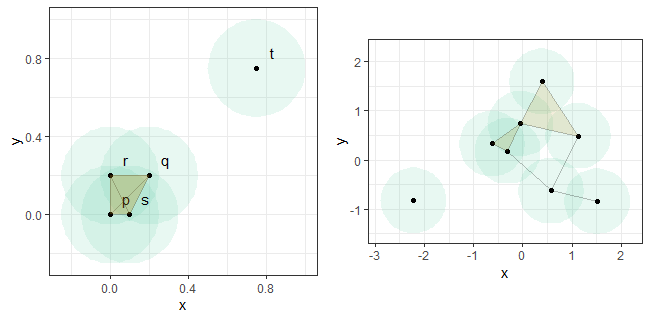
\includegraphics[scale=0.8]{simplicial_complex.png}
    \caption{The figure on the left shows the points $p$, $q$, $r$, $s$ and $t$ with a proximity parameter $\epsilon = 0.5$ and the resulting Rips complex consisting of the tetrahedron $pqrs$, triangles $pqr$, $qrs$, $rsp$,  $pqs$, edges $pq$, $qr$, $rs$, $sp$, $qs$, $pr$ and vertices $p$, $q$, $r$, $s$ and $t$. The figure on the right shows $8$ points and the resulting Rips complex with $\epsilon=4/3$.}
    \label{fig:tetrahedron}
\end{figure}

\subsubsection{Which $\epsilon$?}\label{subsubsec:whicheps}
Given a point cloud of data, the resulting Rips complex depends on the value of $\epsilon$. As such, the question arises which $\epsilon$ is most representative of the structure of the data cloud. For example the point cloud illustrated in Figure~\ref{fig:annulus} lies in an annulus. The figure on the top left shows the Rips complex using $\epsilon = 0.1$. This Rips complex consists of mostly disconnected individual points and a small number of edges. The figure at the top right shows the Rips complex using $\epsilon = 0.3$. This consists of $3$ connected components having edges, triangles, tetrahedrons and possibly other $k$-simplices. The figure at the bottom right shows the Rips complex for $\epsilon = 0.8$, which shows 1 connected component consisting of different $k$-simplices and 1 hole. This Rips complex is desirable from a data analysis point of view as it identifies the annulus well. The figure at the bottom right shows the Rips complex for $\epsilon = 1.5$, which connects everything together and closes up the hole. 

\begin{figure}
    \centering
    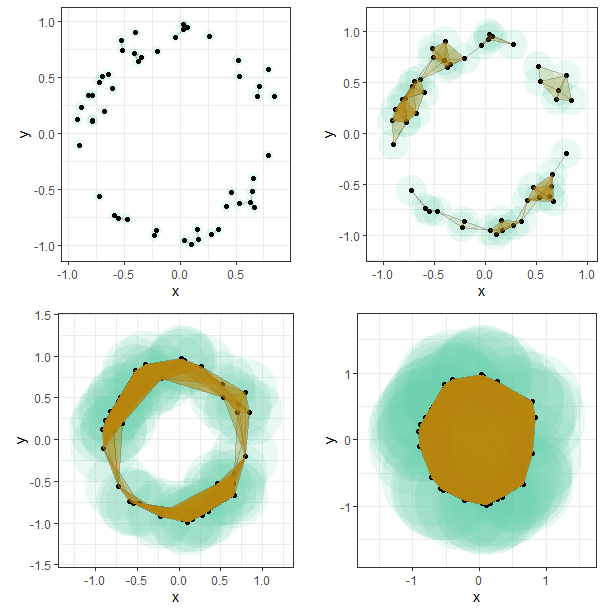
\includegraphics[scale=0.8]{four_plots_diff_radi.png}
    \caption{Rips complexes resulting from different $\epsilon$ values. The figures in the top left, top right, bottom left and bottom right show the Rip complexes resulting from $\epsilon = 0.1, 0.3, 0.8$ and $1.5$ respectively}
    \label{fig:annulus}
\end{figure}

\subsubsection{Persistent homology}\label{persistenthomology}
Keeping the question of best $\epsilon$ aside for a moment, we turn our attention to topological features that has been the focus of persistent homology.  Features that continue for a larger range of $\epsilon$, such as the hole in Figure~\ref{fig:annulus} represent  structural properties of the data that are of interest to us. Informally, the topological construct/feature that counts these holes are called Betti numbers. The Betti number $\beta_k$ counts $k$-dimensional holes of a  simplicial complex. Zero-dimensional holes are connected components and  the number of connected components is given by $\beta_0$.  One-dimensional holes are topological circles and is given by $\beta_1$. Two-dimensional holes are trapped volumes or voids. To study Betti numbers we first define some notation. 

\begin{enumerate}
    \item Introduce simplicial complex - done
    \item Which $\epsilon$ -  sequence of Rips complex
    \item Persistence homology
    \item Barcode - persistence diagram
\end{enumerate}
% =======================================================================
% =======================================================================
\subsection{Extreme value theory}\label{subsec:evt}
This section will introduce extreme value theory and the POT method for exceedences. 
% =======================================================================
% =======================================================================
\subsection{Algorithm lookout}\label{subsec:lookout}
This section will give details of the algorithm. 
\begin{enumerate}
    \item From the persistence diagram selecting a bandwidth
    \item Leave-one-out kernel density estimates using this bandwidth
    \item Take logarithms of KDE values and fit a GPD using POT 
    \item Using these POT parameters, find the probability of seeing the points using log of lookde values
    \item Use a fixed cut off probability of identify outliers
\end{enumerate}
% =======================================================================
% =======================================================================
\section{Simulations}\label{sec:simulations}
% =======================================================================
% =======================================================================
\section{Applications}\label{sec:applications}
% =======================================================================
% =======================================================================
\section{Conclusions}\label{sec:conclusions}
% =======================================================================
% =======================================================================
\section{Supplementary Materials}\label{sec:suppmat}
% =======================================================================

\bibliographystyle{agsm}   % agsm  apalike
 \bibliography{citations}
\end{document}
